\subsection{Non-parametric Mixture of Projected Gammas (NPPG) Model}
\label{method:nppg}
In~\ref{method:mpg}, we fit a finite mixture paradigm on top of the projected
  gamma model.  This raises a legitimate question of how many mixture components
  will be appropriate.  Certainly we could try many numbers of mixture components,
  and via some selection criterion choose an appropriate number.  Alternatively, if
  we were sufficiently gluttons for punishment, we could treat the number of
  components as itself a random variable, and with reversible jump MCMC could
  assemble a finite mixture model where the number of mixture components is
  by the model.  Alternatively, we can forgo that, and use a Dirichlet process
  prior on top of the Projected Gamma distribution.
\begin{equation}
  \label{eqn:nppg}
  \begin{aligned}
    \theta_i &\sim \text{PG}\left(\theta_i\mid ({\bf \alpha}_i, {\bf \beta}_i) \right)\\
    ({\bf \alpha}_i, {\bf \beta}_i) &\sim G_i\\
    G_i &\sim \text{DP}\left(\eta, G_0\left(({\bf \alpha}_i, {\bf \beta}_i)\mid ({\bf a}_{\alpha}, {\bf b}_{\alpha}, {\bf a}_{\beta}, {\bf b}_{\beta}) \right)\right)\\
     ({\bf a}_{\alpha}, {\bf b}_{\alpha}, {\bf a}_{\beta}, {\bf b}_{\beta}) &\sim P\left(({\bf a}_{\alpha}, {\bf b}_{\alpha}, {\bf a}_{\beta}, {\bf b}_{\beta})\right)\\
     \eta &\sim \text{Ga}(a_{\eta},b_{\eta})
  \end{aligned}
\end{equation}
with
\begin{equation*}
    \begin{aligned}
    G_0\left(({\bf \alpha}_i, {\bf \beta}_i)\right) &= \text{Ga}(\alpha_1\mid a_{\alpha_1},b_{\alpha_1})\prod_{j = 2}^d\text{Ga}(\alpha_j\mid a_{\alpha_j}, b_{\alpha_j})\text{Ga}(\beta_j\mid a_{\beta_j}, b_{\beta_j})\\
    P(({\bf a}_{\alpha}, {\bf b}_{\alpha}, {\bf a}_{\beta}, {\bf b}_{\beta})) &= \text{Ga}(a_{\alpha_1})\text{Ga}(b_{\alpha_1})\prod_{j = 2}^d\text{Ga}(a_{\alpha_j})\text{Ga}(b_{\alpha_j})\text{Ga}(a_{\beta_j})\text{Ga}(b_{\beta_j})
    \end{aligned}
\end{equation*}
That is, treat the Projected Gamma distribution as the kernel, with a
  Dirichlet process prior and a product of independent gamma densities as the
  centering distribution.  This has the advantage that the potential number of
  clusters is infinite, the de-facto number of clusters is random.

An obstacle to fitting this model is calculating the prior predictive density,
  which is not available in closed form.  Another obstacle to fitting this
  model, is drawing new random samples for $\alpha_{ij}$.  That is, $\alpha_j$
  for observation $i$.  Posterior samples for $\alpha_j$ in the other finite
  mixture model could be sampled via Metropolis Hastings.  This process takes
  time to reach convergence--there is no assurance that the first draw from
  the sampler for an otherwise empty cluster will be \emph{from the distribution}.
  Every update to the cluster effectively changes the distribution.  As such,
  these draws will have to be perfomed in some other way.  As, after sampling the
  latent radius, we are dealing with independent gammas, we may treat each dimension
  independently.  One solution we might consider would be to use Gaussian quadrature
  approximate the CDF of the distribution, and then sample from it using probability
  integral transform.  This is computationally wasteful, so another idea we
  consider is slice sampling.  The slice sampler is a fair amount slower than
  Metropolis Hastings, but we achieve significantly less correlated draws with no
  tuning of a proposal density.  There is still a starting point that the next draw
  upon, but by some logic we can find a good starting point, and by successively
  sampling some iterations, we can arrive at a draw from the posterior that is
  (effectively) independent of the starting point.

\begin{figure}[h!]
  \centering
  \label{fig:dpmpg}
  \caption{Dirichlet Process Mixture Model with Projected Gamma kernel, independent Gamma priors
          using declustered IVT data.}
  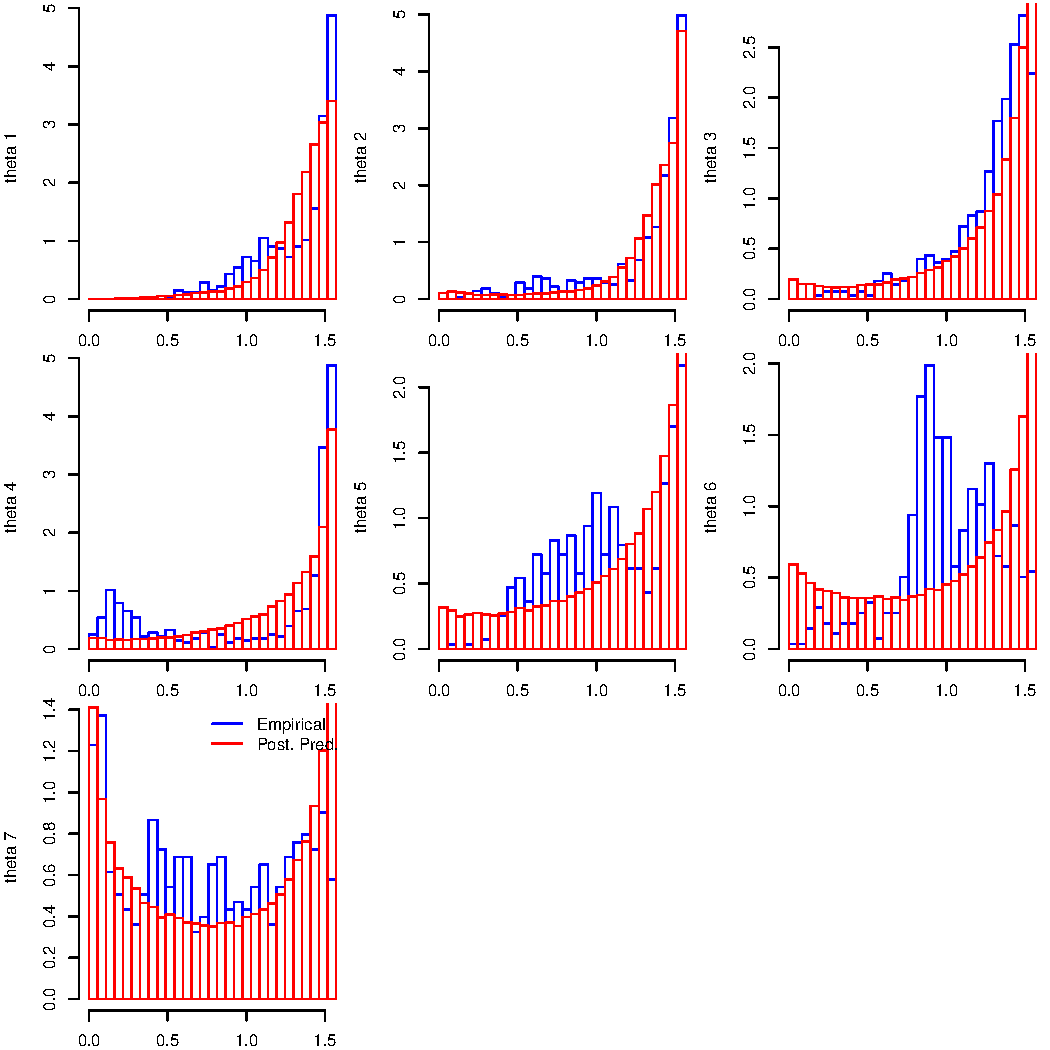
\includegraphics[width=6in]{./images/dpmpg_emp_v_pred_decluster}
\end{figure}

As it turns out, the model as specified above has issues with specifiability, resulting in model
  instability.  The course I took was to fit $b_{\alpha} = b_{\beta} = 1$.  This at least resulted
  in a stable model, but as we can see in Figure~\ref{fig:dpmpg}, the resulting distribution does
  not well match the original data.  The estimates for $a_{\alpha}$ (for all columns) are all
  between $0$ and $0.2$, while the estimates for $a_{\beta}$ (for all columns $> 1$) are stable
  around $20$.  This results, as a prior distribution for possible clusters, in each column having
  a very unstable distribution independent of other columns.  I believe this is why we see such a
  strong prior effect towards independence in Figure~\ref{fig:dpmpg}.

% EOF
